\section*{Организации и их дочерние организации}

Необходимо построить граф из существующих организаций, а так же их дочерних организаций. (Листинг \ref{suborgs})

Используются:
\begin{itemize}
    \item Объект: \href{https://www.wikidata.org/wiki/Q4830453}{business enterprise (Q4830453)} (коммерческая организация)
    \item Свойство: \href{https://www.wikidata.org/wiki/Property:P355}{subsidary (P355)} (дочерняя организации)
\end{itemize}

\begin{lstlisting}[language=SPARQL,label=suborgs,caption=Граф родительских и дочерных организаций]
#subsidary graph
#defaultView:Graph
SELECT ?org ?orgLabel ?subsidary ?subsidaryLabel
WHERE
{
    ?org wdt:P31 wd:Q22687
    ; rdfs:label ?item_label.

    SERVICE wikibase:label { bd:serviceParam wikibase:language "en" }
    OPTIONAL { ?org wdt:P355 ?subsidary. }
    FILTER  (LANG(?item_label) = "en") 
}
\end{lstlisting}

\href{https://query.wikidata.org/#%23neighboring%20countries%20graph%0A%23defaultView%3AGraph%0ASELECT%20%3Forg%20%3ForgLabel%20%3Fsubsidary%20%3FsubsidaryLabel%0AWHERE%0A%7B%0A%20%20%20%20%3Forg%20wdt%3AP31%20wd%3AQ22687%0A%20%20%20%20%3B%20rdfs%3Alabel%20%3Fitem_label%20.%0A%0A%20%20%20%20SERVICE%20wikibase%3Alabel%20%7B%20bd%3AserviceParam%20wikibase%3Alanguage%20%22en%22%20%7D%0A%20%20%20%20OPTIONAL%20%7B%20%3Forg%20wdt%3AP355%20%3Fsubsidary%20.%20%7D%0A%20%20%20%20FILTER%20%20%28LANG%28%3Fitem_label%29%20%3D%20%22en%22%29%20%0A%7D%0A}{SPARQL-запрос}, 428 записей.
	
\begin{figure}[h]
	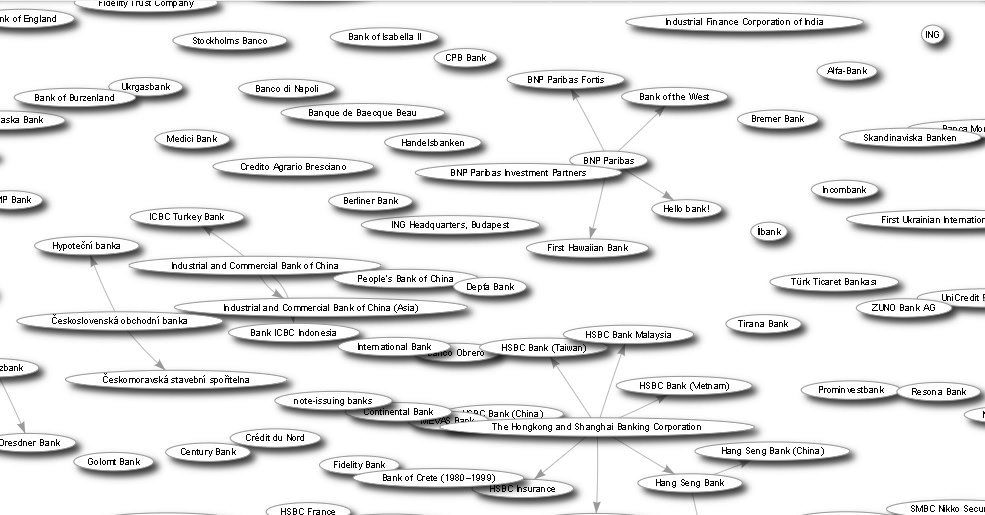
\includegraphics[scale=1.7]{son/son.png}
	\centering
	\caption{Диаграмма дочерних организаций мира}
	\centering
\end{figure}

Полученный граф соседей (рис. 2) состоит из висячих вершин и изолированных. Присутствие изолированных вершин, пожалуй, является недостатком полученного запроса. Необходимо построить такой граф, чтобы в нем отсутствовали эти вершины. (Листинг \ref{suborgs2})


\begin{lstlisting}[language=SPARQL,label=suborgs2,caption=Граф родительских и дочерных организаций без висячих вершин]
#subsidary graph
#defaultView:Graph
SELECT ?org ?orgLabel ?subsidary ?subsidaryLabel
WHERE
{
    ?org wdt:P31 wd:Q22687
    ; rdfs:label ?item_label.
    ?org wdt:P355 ?subsidary. 
  
    SERVICE wikibase:label { bd:serviceParam wikibase:language "en" }

    FILTER  (LANG(?item_label) = "en") 
}
\end{lstlisting}

\href{https://query.wikidata.org/#%23neighboring%20countries%20graph%0A%23defaultView%3AGraph%0ASELECT%20%3Forg%20%3ForgLabel%20%3Fsubsidary%20%3FsubsidaryLabel%0AWHERE%0A%7B%0A%20%20%20%20%3Forg%20wdt%3AP31%20wd%3AQ22687%0A%20%20%20%20%3B%20rdfs%3Alabel%20%3Fitem_label%20.%0A%20%20%20%20%3Forg%20wdt%3AP355%20%3Fsubsidary%20.%20%0A%20%20%0A%20%20%20%20SERVICE%20wikibase%3Alabel%20%7B%20bd%3AserviceParam%20wikibase%3Alanguage%20%22en%22%20%7D%0A%0A%20%20%20%20FILTER%20%20%28LANG%28%3Fitem_label%29%20%3D%20%22en%22%29%20%0A%7D%0A}{SPARQL-запрос}, 55 записей.
